
%% bare_conf.tex
%% V1.4b
%% 2015/08/26
%% by Michael Shell
%% See:
%% http://www.michaelshell.org/
%% for current contact information.
%%
%% This is a skeleton file demonstrating the use of IEEEtran.cls
%% (requires IEEEtran.cls version 1.8b or later) with an IEEE
%% conference paper.
%%
%% Support sites:
%% http://www.michaelshell.org/tex/ieeetran/
%% http://www.ctan.org/pkg/ieeetran
%% and
%% http://www.ieee.org/

%%*************************************************************************
%% Legal Notice:
%% This code is offered as-is without any warranty either expressed or
%% implied; without even the implied warranty of MERCHANTABILITY or
%% FITNESS FOR A PARTICULAR PURPOSE! 
%% User assumes all risk.
%% In no event shall the IEEE or any contributor to this code be liable for
%% any damages or losses, including, but not limited to, incidental,
%% consequential, or any other damages, resulting from the use or misuse
%% of any information contained here.
%%
%% All comments are the opinions of their respective authors and are not
%% necessarily endorsed by the IEEE.
%%
%% This work is distributed under the LaTeX Project Public License (LPPL)
%% ( http://www.latex-project.org/ ) version 1.3, and may be freely used,
%% distributed and modified. A copy of the LPPL, version 1.3, is included
%% in the base LaTeX documentation of all distributions of LaTeX released
%% 2003/12/01 or later.
%% Retain all contribution notices and credits.
%% ** Modified files should be clearly indicated as such, including  **
%% ** renaming them and changing author support contact information. **
%%*************************************************************************


% *** Authors should verify (and, if needed, correct) their LaTeX system  ***
% *** with the testflow diagnostic prior to trusting their LaTeX platform ***
% *** with production work. The IEEE's font choices and paper sizes can   ***
% *** trigger bugs that do not appear when using other class files.       ***                          ***
% The testflow support page is at:
% http://www.michaelshell.org/tex/testflow/



\documentclass[conference]{IEEEtran}
% Some Computer Society conferences also require the compsoc mode option,
% but others use the standard conference format.
%
% If IEEEtran.cls has not been installed into the LaTeX system files,
% manually specify the path to it like:
% \documentclass[conference]{../sty/IEEEtran}


\usepackage{epsfig}
\usepackage{algorithm}
\usepackage{algorithmicx}
\usepackage{algpseudocode}
\usepackage{CJK}
\usepackage{indentfirst}
\usepackage{amsmath}
\usepackage{url}

\renewcommand{\algorithmicrequire}{ \textbf{Input:}}      %Use Input in the format of Algorithm
\renewcommand{\algorithmicensure}{ \textbf{Output:}}     %UseOutput in the format of Algorithm



% Some very useful LaTeX packages include:
% (uncomment the ones you want to load)


% *** MISC UTILITY PACKAGES ***
%
%\usepackage{ifpdf}
% Heiko Oberdiek's ifpdf.sty is very useful if you need conditional
% compilation based on whether the output is pdf or dvi.
% usage:
% \ifpdf
%   % pdf code
% \else
%   % dvi code
% \fi
% The latest version of ifpdf.sty can be obtained from:
% http://www.ctan.org/pkg/ifpdf
% Also, note that IEEEtran.cls V1.7 and later provides a builtin
% \ifCLASSINFOpdf conditional that works the same way.
% When switching from latex to pdflatex and vice-versa, the compiler may
% have to be run twice to clear warning/error messages.






% *** CITATION PACKAGES ***
%
%\usepackage{cite}
% cite.sty was written by Donald Arseneau
% V1.6 and later of IEEEtran pre-defines the format of the cite.sty package
% \cite{} output to follow that of the IEEE. Loading the cite package will
% result in citation numbers being automatically sorted and properly
% "compressed/ranged". e.g., [1], [9], [2], [7], [5], [6] without using
% cite.sty will become [1], [2], [5]--[7], [9] using cite.sty. cite.sty's
% \cite will automatically add leading space, if needed. Use cite.sty's
% noadjust option (cite.sty V3.8 and later) if you want to turn this off
% such as if a citation ever needs to be enclosed in parenthesis.
% cite.sty is already installed on most LaTeX systems. Be sure and use
% version 5.0 (2009-03-20) and later if using hyperref.sty.
% The latest version can be obtained at:
% http://www.ctan.org/pkg/cite
% The documentation is contained in the cite.sty file itself.






% *** GRAPHICS RELATED PACKAGES ***
%
\ifCLASSINFOpdf
  % \usepackage[pdftex]{graphicx}
  % declare the path(s) where your graphic files are
  % \graphicspath{{../pdf/}{../jpeg/}}
  % and their extensions so you won't have to specify these with
  % every instance of \includegraphics
  % \DeclareGraphicsExtensions{.pdf,.jpeg,.png}
\else
  % or other class option (dvipsone, dvipdf, if not using dvips). graphicx
  % will default to the driver specified in the system graphics.cfg if no
  % driver is specified.
  % \usepackage[dvips]{graphicx}
  % declare the path(s) where your graphic files are
  % \graphicspath{{../eps/}}
  % and their extensions so you won't have to specify these with
  % every instance of \includegraphics
  % \DeclareGraphicsExtensions{.eps}
\fi
% graphicx was written by David Carlisle and Sebastian Rahtz. It is
% required if you want graphics, photos, etc. graphicx.sty is already
% installed on most LaTeX systems. The latest version and documentation
% can be obtained at: 
% http://www.ctan.org/pkg/graphicx
% Another good source of documentation is "Using Imported Graphics in
% LaTeX2e" by Keith Reckdahl which can be found at:
% http://www.ctan.org/pkg/epslatex
%
% latex, and pdflatex in dvi mode, support graphics in encapsulated
% postscript (.eps) format. pdflatex in pdf mode supports graphics
% in .pdf, .jpeg, .png and .mps (metapost) formats. Users should ensure
% that all non-photo figures use a vector format (.eps, .pdf, .mps) and
% not a bitmapped formats (.jpeg, .png). The IEEE frowns on bitmapped formats
% which can result in "jaggedy"/blurry rendering of lines and letters as
% well as large increases in file sizes.
%
% You can find documentation about the pdfTeX application at:
% http://www.tug.org/applications/pdftex





% *** MATH PACKAGES ***
%
%\usepackage{amsmath}
% A popular package from the American Mathematical Society that provides
% many useful and powerful commands for dealing with mathematics.
%
% Note that the amsmath package sets \interdisplaylinepenalty to 10000
% thus preventing page breaks from occurring within multiline equations. Use:
%\interdisplaylinepenalty=2500
% after loading amsmath to restore such page breaks as IEEEtran.cls normally
% does. amsmath.sty is already installed on most LaTeX systems. The latest
% version and documentation can be obtained at:
% http://www.ctan.org/pkg/amsmath





% *** SPECIALIZED LIST PACKAGES ***
%
%\usepackage{algorithmic}
% algorithmic.sty was written by Peter Williams and Rogerio Brito.
% This package provides an algorithmic environment fo describing algorithms.
% You can use the algorithmic environment in-text or within a figure
% environment to provide for a floating algorithm. Do NOT use the algorithm
% floating environment provided by algorithm.sty (by the same authors) or
% algorithm2e.sty (by Christophe Fiorio) as the IEEE does not use dedicated
% algorithm float types and packages that provide these will not provide
% correct IEEE style captions. The latest version and documentation of
% algorithmic.sty can be obtained at:
% http://www.ctan.org/pkg/algorithms
% Also of interest may be the (relatively newer and more customizable)
% algorithmicx.sty package by Szasz Janos:
% http://www.ctan.org/pkg/algorithmicx




% *** ALIGNMENT PACKAGES ***
%
%\usepackage{array}
% Frank Mittelbach's and David Carlisle's array.sty patches and improves
% the standard LaTeX2e array and tabular environments to provide better
% appearance and additional user controls. As the default LaTeX2e table
% generation code is lacking to the point of almost being broken with
% respect to the quality of the end results, all users are strongly
% advised to use an enhanced (at the very least that provided by array.sty)
% set of table tools. array.sty is already installed on most systems. The
% latest version and documentation can be obtained at:
% http://www.ctan.org/pkg/array


% IEEEtran contains the IEEEeqnarray family of commands that can be used to
% generate multiline equations as well as matrices, tables, etc., of high
% quality.




% *** SUBFIGURE PACKAGES ***
%\ifCLASSOPTIONcompsoc
%  \usepackage[caption=false,font=normalsize,labelfont=sf,textfont=sf]{subfig}
%\else
%  \usepackage[caption=false,font=footnotesize]{subfig}
%\fi
% subfig.sty, written by Steven Douglas Cochran, is the modern replacement
% for subfigure.sty, the latter of which is no longer maintained and is
% incompatible with some LaTeX packages including fixltx2e. However,
% subfig.sty requires and automatically loads Axel Sommerfeldt's caption.sty
% which will override IEEEtran.cls' handling of captions and this will result
% in non-IEEE style figure/table captions. To prevent this problem, be sure
% and invoke subfig.sty's "caption=false" package option (available since
% subfig.sty version 1.3, 2005/06/28) as this is will preserve IEEEtran.cls
% handling of captions.
% Note that the Computer Society format requires a larger sans serif font
% than the serif footnote size font used in traditional IEEE formatting
% and thus the need to invoke different subfig.sty package options depending
% on whether compsoc mode has been enabled.
%
% The latest version and documentation of subfig.sty can be obtained at:
% http://www.ctan.org/pkg/subfig




% *** FLOAT PACKAGES ***
%
%\usepackage{fixltx2e}
% fixltx2e, the successor to the earlier fix2col.sty, was written by
% Frank Mittelbach and David Carlisle. This package corrects a few problems
% in the LaTeX2e kernel, the most notable of which is that in current
% LaTeX2e releases, the ordering of single and double column floats is not
% guaranteed to be preserved. Thus, an unpatched LaTeX2e can allow a
% single column figure to be placed prior to an earlier double column
% figure.
% Be aware that LaTeX2e kernels dated 2015 and later have fixltx2e.sty's
% corrections already built into the system in which case a warning will
% be issued if an attempt is made to load fixltx2e.sty as it is no longer
% needed.
% The latest version and documentation can be found at:
% http://www.ctan.org/pkg/fixltx2e


%\usepackage{stfloats}
% stfloats.sty was written by Sigitas Tolusis. This package gives LaTeX2e
% the ability to do double column floats at the bottom of the page as well
% as the top. (e.g., "\begin{figure*}[!b]" is not normally possible in
% LaTeX2e). It also provides a command:
%\fnbelowfloat
% to enable the placement of footnotes below bottom floats (the standard
% LaTeX2e kernel puts them above bottom floats). This is an invasive package
% which rewrites many portions of the LaTeX2e float routines. It may not work
% with other packages that modify the LaTeX2e float routines. The latest
% version and documentation can be obtained at:
% http://www.ctan.org/pkg/stfloats
% Do not use the stfloats baselinefloat ability as the IEEE does not allow
% \baselineskip to stretch. Authors submitting work to the IEEE should note
% that the IEEE rarely uses double column equations and that authors should try
% to avoid such use. Do not be tempted to use the cuted.sty or midfloat.sty
% packages (also by Sigitas Tolusis) as the IEEE does not format its papers in
% such ways.
% Do not attempt to use stfloats with fixltx2e as they are incompatible.
% Instead, use Morten Hogholm'a dblfloatfix which combines the features
% of both fixltx2e and stfloats:
%
% \usepackage{dblfloatfix}
% The latest version can be found at:
% http://www.ctan.org/pkg/dblfloatfix




% *** PDF, URL AND HYPERLINK PACKAGES ***
%
%\usepackage{url}
% url.sty was written by Donald Arseneau. It provides better support for
% handling and breaking URLs. url.sty is already installed on most LaTeX
% systems. The latest version and documentation can be obtained at:
% http://www.ctan.org/pkg/url
% Basically, \url{my_url_here}.




% *** Do not adjust lengths that control margins, column widths, etc. ***
% *** Do not use packages that alter fonts (such as pslatex).         ***
% There should be no need to do such things with IEEEtran.cls V1.6 and later.
% (Unless specifically asked to do so by the journal or conference you plan
% to submit to, of course. )


% correct bad hyphenation here
\hyphenation{op-tical net-works semi-conduc-tor}


\begin{document}
%
% paper title
% Titles are generally capitalized except for words such as a, an, and, as,
% at, but, by, for, in, nor, of, on, or, the, to and up, which are usually
% not capitalized unless they are the first or last word of the title.
% Linebreaks \\ can be used within to get better formatting as desired.
% Do not put math or special symbols in the title.
\title{A Web of Things based device-adaptive service composition framework}


% author names and affiliations
% use a multiple column layout for up to three different
% affiliations
\author{\IEEEauthorblockN{Junjie Mao}
\IEEEauthorblockA{School of Software\\
Shanghai Jiao Tong University\\
Shanghai, China\\
Email: charlie-white@sjtu.edu.cn}}

% conference papers do not typically use \thanks and this command
% is locked out in conference mode. If really needed, such as for
% the acknowledgment of grants, issue a \IEEEoverridecommandlockouts
% after \documentclass

% for over three affiliations, or if they all won't fit within the width
% of the page, use this alternative format:
% 
%\author{\IEEEauthorblockN{Michael Shell\IEEEauthorrefmark{1},
%Homer Simpson\IEEEauthorrefmark{2},
%James Kirk\IEEEauthorrefmark{3}, 
%Montgomery Scott\IEEEauthorrefmark{3} and
%Eldon Tyrell\IEEEauthorrefmark{4}}
%\IEEEauthorblockA{\IEEEauthorrefmark{1}School of Electrical and Computer Engineering\\
%Georgia Institute of Technology,
%Atlanta, Georgia 30332--0250\\ Email: see http://www.michaelshell.org/contact.html}
%\IEEEauthorblockA{\IEEEauthorrefmark{2}Twentieth Century Fox, Springfield, USA\\
%Email: homer@thesimpsons.com}
%\IEEEauthorblockA{\IEEEauthorrefmark{3}Starfleet Academy, San Francisco, California 96678-2391\\
%Telephone: (800) 555--1212, Fax: (888) 555--1212}
%\IEEEauthorblockA{\IEEEauthorrefmark{4}Tyrell Inc., 123 Replicant Street, Los Angeles, California 90210--4321}}




% use for special paper notices
%\IEEEspecialpapernotice{(Invited Paper)}




% make the title area
\maketitle

% As a general rule, do not put math, special symbols or citations
% in the abstract
\begin{abstract}
In WoT environment, smart things provide RESTful services to expose their resources and operations. There are lots of smart things that offer the same functionalities but have different service interfaces. Because of the high coupling between device service instances and process specifications like BPEL, the cost of reusing a BPEL specification between different device environments is very high. We propose a device-adaptive service composition framework for WoT environment, in order to help users to apply the business process and service composition technologies more conveniently. In the framework, we design an activity description model, which is a semantic description for business activities, to overcome the shortcoming of directly binding the process and the service. Then, a matching mechanism between the model and the WADL of device services is proposed to select candidate services for the composition. Furthermore, we represent the matching result in a general service model, with which the source code of the general service can be automatically generated. The general service is a unified encapsulation for device services that match the functionalities of business activity. So user can interact with the general service instead of the origin services on the device, which decouple the process specification and the actual device services. A case study is offered to illustrate how to apply our framework in a intelligent charging pile sharing platform. 
\end{abstract}
\bigskip
\begin{IEEEkeywords}
WoT;service composition;
\end{IEEEkeywords}

% no keywords




% For peer review papers, you can put extra information on the cover
% page as needed:
% \ifCLASSOPTIONpeerreview
% \begin{center} \bfseries EDICS Category: 3-BBND \end{center}
% \fi
%
% For peerreview papers, this IEEEtran command inserts a page break and
% creates the second title. It will be ignored for other modes.
\IEEEpeerreviewmaketitle



%\section{Introduction}
% no \IEEEPARstart
%This demo file is intended to serve as a ``starter file''
%for IEEE conference papers produced under \LaTeX\ using
%IEEEtran.cls version 1.8b and later.
% You must have at least 2 lines in the paragraph with the drop letter
% (should never be an issue)
%I wish you the best of success.

%\hfill mds1
 
%\hfill August 26, 2015

%\subsection{Subsection Heading Here}
%Subsection text here.


%\subsubsection{Subsubsection Heading Here}
%Subsubsection text here.


% An example of a floating figure using the graphicx package.
% Note that \label must occur AFTER (or within) \caption.
% For figures, \caption should occur after the \includegraphics.
% Note that IEEEtran v1.7 and later has special internal code that
% is designed to preserve the operation of \label within \caption
% even when the captionsoff option is in effect. However, because
% of issues like this, it may be the safest practice to put all your
% \label just after \caption rather than within \caption{}.
%
% Reminder: the "draftcls" or "draftclsnofoot", not "draft", class
% option should be used if it is desired that the figures are to be
% displayed while in draft mode.
%
%\begin{figure}[!t]
%\centering
%\includegraphics[width=2.5in]{myfigure}
% where an .eps filename suffix will be assumed under latex, 
% and a .pdf suffix will be assumed for pdflatex; or what has been declared
% via \DeclareGraphicsExtensions.
%\caption{Simulation results for the network.}
%\label{fig_sim}
%\end{figure}

% Note that the IEEE typically puts floats only at the top, even when this
% results in a large percentage of a column being occupied by floats.


% An example of a double column floating figure using two subfigures.
% (The subfig.sty package must be loaded for this to work.)
% The subfigure \label commands are set within each subfloat command,
% and the \label for the overall figure must come after \caption.
% \hfil is used as a separator to get equal spacing.
% Watch out that the combined width of all the subfigures on a 
% line do not exceed the text width or a line break will occur.
%
%\begin{figure*}[!t]
%\centering
%\subfloat[Case I]{\includegraphics[width=2.5in]{box}%
%\label{fig_first_case}}
%\hfil
%\subfloat[Case II]{\includegraphics[width=2.5in]{box}%
%\label{fig_second_case}}
%\caption{Simulation results for the network.}
%\label{fig_sim}
%\end{figure*}
%
% Note that often IEEE papers with subfigures do not employ subfigure
% captions (using the optional argument to \subfloat[]), but instead will
% reference/describe all of them (a), (b), etc., within the main caption.
% Be aware that for subfig.sty to generate the (a), (b), etc., subfigure
% labels, the optional argument to \subfloat must be present. If a
% subcaption is not desired, just leave its contents blank,
% e.g., \subfloat[].


% An example of a floating table. Note that, for IEEE style tables, the
% \caption command should come BEFORE the table and, given that table
% captions serve much like titles, are usually capitalized except for words
% such as a, an, and, as, at, but, by, for, in, nor, of, on, or, the, to
% and up, which are usually not capitalized unless they are the first or
% last word of the caption. Table text will default to \footnotesize as
% the IEEE normally uses this smaller font for tables.
% The \label must come after \caption as always.
%
%\begin{table}[!t]
%% increase table row spacing, adjust to taste
%\renewcommand{\arraystretch}{1.3}
% if using array.sty, it might be a good idea to tweak the value of
% \extrarowheight as needed to properly center the text within the cells
%\caption{An Example of a Table}
%\label{table_example}
%\centering
%% Some packages, such as MDW tools, offer better commands for making tables
%% than the plain LaTeX2e tabular which is used here.
%\begin{tabular}{|c||c|}
%\hline
%One & Two\\
%\hline
%Three & Four\\
%\hline
%\end{tabular}
%\end{table}


% Note that the IEEE does not put floats in the very first column
% - or typically anywhere on the first page for that matter. Also,
% in-text middle ("here") positioning is typically not used, but it
% is allowed and encouraged for Computer Society conferences (but
% not Computer Society journals). Most IEEE journals/conferences use
% top floats exclusively. 
% Note that, LaTeX2e, unlike IEEE journals/conferences, places
% footnotes above bottom floats. This can be corrected via the
% \fnbelowfloat command of the stfloats package.




%******************paper start here****************************


\section{Introduction}
\label{Introduction}
During the last decade, the Internet of Things(IoT) technologies have been much more widely applied in both enterprise manufacturing and people's daily life. Concepts like Smart City, Intelligent Manufacturing, E-health are all closely bound up to IOT technologies. As increasing numbers of IoT devices (e.g., sensors, actuators, embeded devices, RFID) are getting connected to the World Wide Web(WWW)\cite{guinard2011internet}, the Web of Things(WoT) architecture offers us a new platform which enables us to manage and integrate the smart things in a much easier way with looser coupling and better scalability. 

Different from the IoT that focuses on the network layer connectivity between physical devices in various constrained networking environments, the WoT focuses on integrating smart things into the application layer, the top level of the Internet. Web servers are embeded into smart things and the physical resources are exposed to the Internet as RESTful Web Services\cite{guinard2010resource}. Compared with the traditional heavyweight Web Service technologies based on standards such as SOAP, WSDL, and UDDI , RESTful Web Service can be accessed in a easier way through HTTP or HTTPS protocol. In the RESTful architecture, all the resources are identified and  encapsulated uniquely through the Universal Resource Identifiers(URIs), which can effectively solve the problems caused by the variability of data structure and data transmission mode between different devices and make the information exchange become more efficient through different programming languages, different platforms, and different devices\cite{pautasso2008restful}.  

As massive smart things are accessable in WoT environment, simple service invocation can hardly meet the requirement of increasingly complex applications. Therefore, our demand for business process management and service composition technologies in WoT environment is becoming very urgent. Business Process Execution Language(BPEL) is one of the most frequently used process definition standard\cite{jordan2003web}. BPEL binds business activities and Web Services and control the business processes with workflow, so as to execute complex business processes by service composition. However, such bindings refer actual service instances instead of service  interfaces during the process definition phase, which will make high coupling between processes and devices in WoT. There are lots of smart things that offer the same functionalities but were produced by different manufacturers, which means that the Application Programming Interface(API), parameters, and constraints of those smart things are different. For example, there are hundreds of different models of charging pile produced by nearly a hundred charging pile manufacturers. Because of the variety of the device interface, it’s very complicated to reuse a BPEL specification between different device environment, and a simple replacement of devices may lead to the rewriting of the entire specification. 

In order to solve the defects above and allow users to define and make use of the business process management and service composition technologies more conveniently, we propose a device-adaptive service composition framework for WoT environment. In the framework, we design an activity description model and a general service model. In the activity description model, by using ontology to construct a semantic extension of a business activity in BPEL, we can overcome the shortcoming of directly binding the process and the service and  make the process specification more reusable with the more abstract definition. Then, a matching mechanism between the model and the Web Application Description Language(WADL) is proposed to select available services from all the services of the device. The matching result is represented by a general service model, which contains the references to actual service instances. According to the general service model, source code of the general service can be automatically generated. The source code  will be deployed on the device to publish the composited service for the business activity, so that users only need to interact with such service during the process execution and should pay no attention to the origin services on the device, which decouple the process specification and the actual device services. Through this approach, once the business activity should be reused in other device environment, we can generate the general services on the new devices automatically instead of redefine the entire process. 

The remainder of the paper is organized as follows. In Section~\ref{Related Work}, we introduce some existing semantic related business process and service composition technologies, and make a comparision with our approach. The overall architecture of our framework is briefly presented in Section~\ref{Framework}. In Section~\ref{Approach}, we describe our activity description model, general service model, algorithms for matching and code generation in detail. Then, there is a case study about applying our framework in a scene of intelligent charging piles in Section~\ref{CaseStudy} and we draw our conclusions in Section~\ref{Conclusion}. 


\section{Related Work}
\label{Related Work}
To integrate traditional enterprise services and wireless sensor networks, [6] proposes a lightweight approach following the success of Web 2.0 "mashups”, proposing and implementing a collection of RESTful services to expose sensor nodes to web resources so that all the nodes become part of a ‘Web of Thing’ and interact with existing nodes to compose their services. [7] combines the above work with an AutoWot platform, which offers a generic way to model Web resources and build Web components in order to facilitate the integration of smart devices into web.The integration, however, is based on particular service instances for service composition, failing to describe the composition from a abstract level. 

[8] designs a WebPlug framework to strengthen the combination of real physical devices with virtual resources. In the framework, users can get access to physical resources by URL as well as the MetaURL defined by framework to obtain the related information about the device. For example adding “@history” after the URL of the device can archive the history information of this resource.SemSense proposed by [9] is composed of data collection module, storage module, semantic module and release module. Data are first collected from physical sensor, enriched by semantic annotation using LinkedData and finally published. Both approaches above are limited to annotating the resources, and are lack of the coordination among devices and services. 

For the semantic extension of process description language, traditional methods like BPEL have a low precision about the similarity between conceptual similar service, due to the strict matching strategy[14]. WSDL-S[15] can't distinguish between service type(concept) and service instance(individual), as it's restriction in the expansion of the service concept. Likewise, in OWL-S [16], there is no significant difference between the process instance (the actual combination of services) and conceptual process (only relating to the concept of services). 

In [19], researchers propose a RESTful service composition modeling method based on UML, using a conceptual resource model to describe the static composition structure. Besides, a state machine is used to represent the behavior information of the HTTP methods like PUT and POST. But the drawback is that it is hard to implement the actual service composition based on the model. 

[20] proposes an approach termed as Web Service Resource Bundle(WSRB), considering the dependencies between the candidate services and binding those services during the invocation from the client, which offers a novel runtime compositing concept. But WSRB focuses on the fixed and predefined composition, failing to support the dynamic composition based on the business requirement. 

The above literature survey shows that it is hard to directly apply existing business process and service composition technologies to WoT. 


\section{Framework}
\label{Framework}
\begin{figure}[!t]
\centering
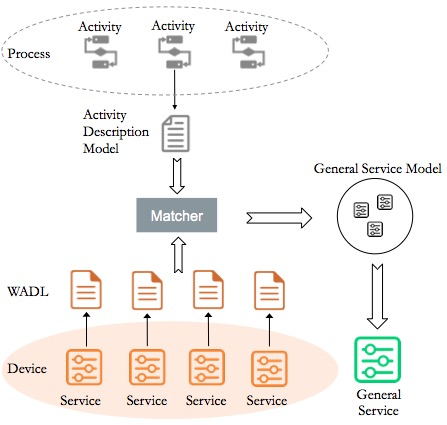
\includegraphics[width=1.0\linewidth]{./graph/framework}
% where an .eps filename suffix will be assumed under latex, 
% and a .pdf suffix will be assumed for pdflatex; or what has been declared
%via \DeclareGraphicsExtensions.
\caption{Overall architecture for the framework.}
\label{fig_framework}
\end{figure}
The overall architecture of our framework is shown in Fig.~\ref{fig_framework}. In a business process, each activity is bound to an activity description model. The model is defined in a XML structure by RDF, which is a recommended semantic modeling metadata. The model provides ontological annotations for the binding activity abouts it's functionalities and messages. In order to reduce extra work for modeling, an Eclipse plugin is offered to help users to construct the models more effectively after the process is  defined. 

The matcher is the central component. Once the device envrionment is changed, users can upload the WADL description of the services of the new device and the activity description model to the matcher. A semantic-based matching mechanism is executed to find suitable service composition strategy, and the matching result will be presented in a general service model. 

The general service model is consist of two part: (1) description of the general service, including resource path, request method, request and response parameters, and (2)actual service instances to composite and parameters mappings. On the basis of the model, a general service can be automatically generated. For the invoker of the general service, the service provides a device-independent request interface, which means that the invoker is able to call the general services from different devices that have the same capabilities of the process activity and don't need to modify the HTTP request at all. 

\section{Approach}
\label{Approach}
\subsection{Activity Description Model}
When expressing a business process in BPEL, we are essentially defining a composite relationship of existing services. In BPEL, the $<invoke>$ primitive is used to represent the common task that invoke a Web Service instance. Nevertheless, in WoT, such kind of direct service binding may lead to several limitations. Because device environment is changeable and devices with similar functionalities offer different services, the cost of maintaining the process specification is very high. 

In the context of intelligent charging pill, the capabilities of the devices are exactly the same, but the process definition cannot be shared. The invoke bindings of the process must be rewritten to adapt the service interface of different charging pill. 

To address such limitations, a more abstract and more generate workflow definition is a feasible solution. We propose an activity description model, to attach ontological description for the business activity. The model can be represented as a tuple, 
\begin{equation}
	{AD} = \textless\textbf{DM}, \textbf{IM}, \textbf{OM}, \textbf{BF}\textgreater
\end{equation}where \textbf{DM}, \textbf{IM}, \textbf{OM}, \textbf{BF} denote domain, input messages, output messages, and business functionalities. Domain represents the device environment of current activity. Input messages and output messages contain variables with identity and data type. Business functionalities are consist of several verb-object constructions, which describe the business activity from a resource and operation perspective. 

\begin{figure}[!t]
\centering
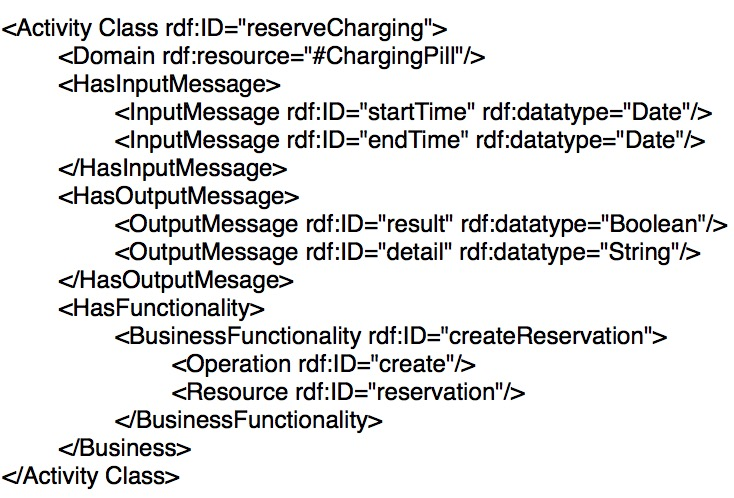
\includegraphics[width=1.0\linewidth]{./graph/activitydescriptionmodeldemo}
% where an .eps filename suffix will be assumed under latex, 
% and a .pdf suffix will be assumed for pdflatex; or what has been declared
%via \DeclareGraphicsExtensions.
\caption{Sample description of a reservation activity.}
\label{fig_activitydescriptionmodeldemo}
\end{figure}

In lots of semantic based service composition technologies, researchers perfer to take advantage of Input, Output, Pre-condition, Effect(IOPE) as the basis of service description and the critical parameters of the service matchmaking calculation\cite{syu2012survey}\cite{lee2013service}. However, in our model, we choose the simpler verb-object construction instead of the Pre-condition and Effect(PE), because: (1) Most of the RESTful Web Services in WoT are simple resource operations; (2) Defining a PE is much more sophisticated than defining a verb-object construction; (3) To campare with the semantic similarity calculation(between the functionality and the resource URL), the matchmaking calculation on PE is inefficiency. 

\begin{figure}[!b]
\centering
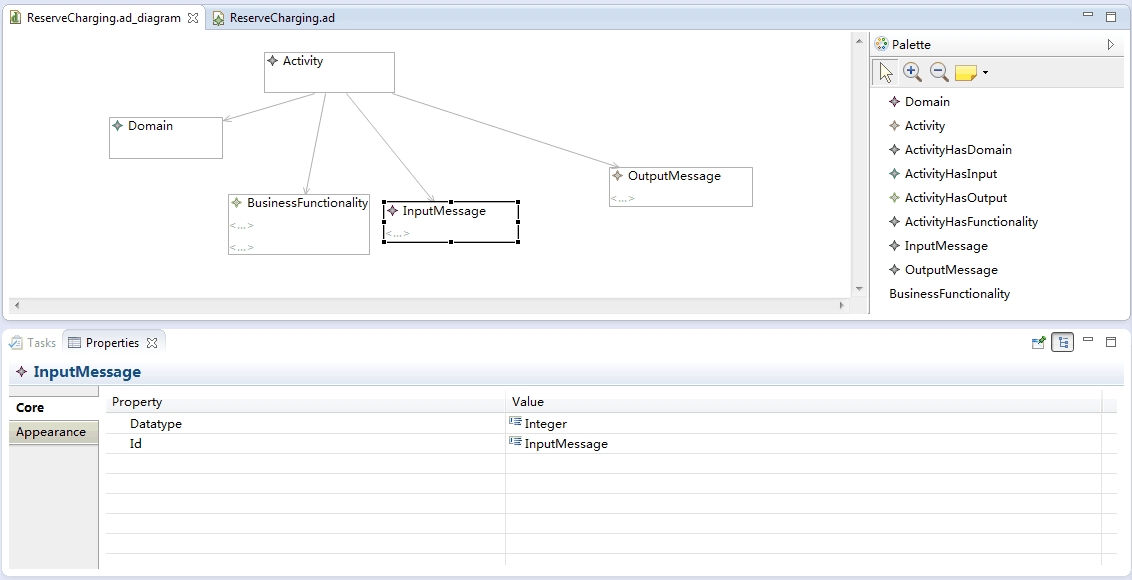
\includegraphics[width=1.0\linewidth]{./graph/eclipseplugin}
% where an .eps filename suffix will be assumed under latex, 
% and a .pdf suffix will be assumed for pdflatex; or what has been declared
%via \DeclareGraphicsExtensions.
\caption{A graphical modeling tool for the activity description model.}
\label{fig_eclipseplugin}
\end{figure}

Taking the charging pill as an example, an activity description model instance about the "reserveCharging" activity is shown in Fig.~\ref{fig_activitydescriptionmodeldemo}. The core resource operation of this activity is creating a reservation for a charging pill, which takes $startTime$ and $endTime$ as constructor arguments, and $result$ and $detail$ are returned to show whether the create operation is success or not and a detailed reason for the failure. 

Also, we try to provide a convenient and efficient way for users to specify their workflow in our model. As is shown in Fig.~\ref{fig_eclipseplugin}, a graphical modeling tool is afforded in the form of an Eclipse plugin. With such plugin, users can create an activity description model file for a business activity, drag and drop model nodes to the canvas, and fulfil the properties in an editing frame, just like defining a BPEL schema with the BPEL Designer for Eclipse. 

\begin{figure}[!t]
\centering
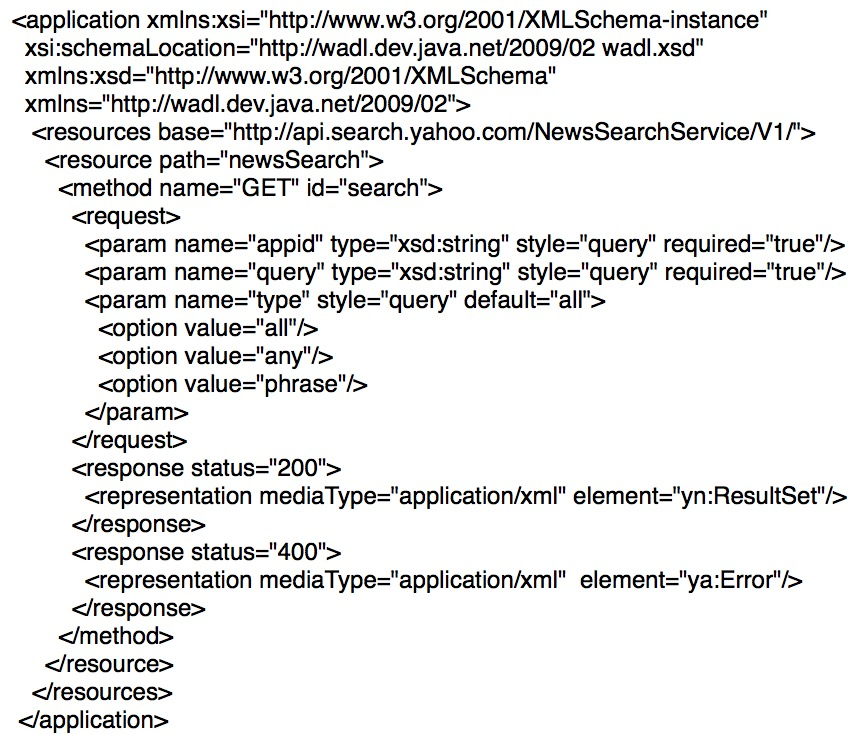
\includegraphics[width=1.0\linewidth]{./graph/wadl}
% where an .eps filename suffix will be assumed under latex, 
% and a .pdf suffix will be assumed for pdflatex; or what has been declared
%via \DeclareGraphicsExtensions.
\caption{Sample description of a reservation activity.}
\label{fig_wadl}
\end{figure}

\subsection{Matching Strategy}
In this subsection, we will give a detailed introduction to our matching strategy between our activity description model and device services. The WADL documents of those servics will be 
utilized for seeking out appropriate services that match the business functionality description. 

In actual Internet applications, capabilities provided by RESTful services are far more complex than pure resource operations, and the form of data exchange is more in nested structure like JSON and XML than basic data types like string or integer. But, as mentioned above, in the WOT environment, most RESTful services provided by smart devices are simple  resource operations, which will not be too complicated. Therefore, our matching strategy will pay more attention to the  equivalence of resources and operations, so that the complexity of the matching can be reduced to get a higher matching efficiency. 

Fig.~\ref{fig_wadl} shows a common WADL file example from Wikipedia. Generally speaking, a RESTful service denote an operation to a resource. Information about what resource the service has and how to invode the service is contained in the WADL document throught following nodes: (1) A $resources$ node is seen as a container for the $resource$ nodes, presenting the basic URL address of it's resources; (2) A $resource$ node specifies the resource to operate in the service with a path attribute; (3) A $method$ node is embodied in a $resource$ node to show the HTTP request method (e.g., GET, PUT, POST, DELETE) that can be accepted by the service, which also stand for the operation towards resource; (4) A $request$ node is a container for the $param$ nodes; (5) A $param$ node describes an input parameter of the service, including the data type of the parameter and whether such parameter is necessary or not. 

According to the WADL structure above, we can find that information about resource and operation of a service is in the $resource$ node and the $method$ node. In the $resource$ node, the path attribute is generally constitutive of a group of simple words, such as user/register and user/password/reset. Such group of words can always be divided into two part, a series of nouns to locate the URI of the resource, and a verb to appoint the operation on it. 

However, in some special cases, there might be no verb in a URL path. We often use a user/\{userid\}/orders  path to indicate the action that fetch all the orders of a user. In this circumstance, the operation information should be complemented by the HTTP request method in the $method$ node. There are eight HTTP request methods defined in the HTTP/1.1 specification, while the GET, PUT, POST, DELETE methods are the most commonly used ones. Owing to the HTTP specification, such methods have well known and dependable semantic meaning. A request with the GET method is always used for retrieving data. Consequently, for URL like user/\{userId\}/orders with the GET method, we can infer that it is a query service and the operation on the resource can be annotated as a "search" or a "get". Similarly, with a PUT or POST method, we can associate a "create" operation with a resource that have no specified identifier (e.g., userId), and an "update" operation with a resource that have specified identifier. 

After recognizing the resource and the operation of a service, we can refine the semantic similarity between the service and the business functionality defined in our activity description model. The similarity calculation formula is:
\begin{equation}
	Sim(f,s) = S(r_f,r_s) \times S(o_f,o_s)
\end{equation}
In (2), $f$ and $s$ denote the functionality(described in the model) and the service. $S(r_f,r_s)$ is the similarity between the resources in the functionality and the service, which can be predefined in an ontology repository or be retrieved in the WordNet\cite{wordnet}. 

Due to the limitation of performance in smart devices, we can assume that there will not be two services in one device that offer resemble operations on the same resource. Therefore, a conclusion can be drawn that the service with the highest similarity is the matching service. The algorithm for finding the matching service is defined in Algorithm~\ref{al_matching}. 
 \begin{algorithm}
        \caption{Find Matching Service}
        \begin{algorithmic}[1] 
            \Require resource and operation of a functionality description $R_f$, $O_f$, and services of a smart device $S = \{ s_1, s_2,\cdots,s_n\}$
            \Ensure the matching service to the functionality description
                   \For {each service $s_i$ in $S$}
                   	   \State Let $W_i$ be the WADL description of $s_i$
  					   \State Let $path$ be the path attribute of the resource node in $W_i$
  					   \State Split $path$ to get a word vector $WORD_i$
  					   \State Let $R_{si}$ and $O_{si}$ be the last noun and verb in the vector $WORD_i$
  					   \If {$O_{si}$ is null}
  					   		\State Complement the $O_{si}$ based on the $method$ node in $W_i$
  					   \EndIf
  					   \State $SIM_{si} \leftarrow Sim(R_f,R_{si}) \times Sim(O_f,O_{si})$ //$Sim(a,b)$ is the API to calculate the similarity between $a$ and $b$
				   \EndFor
				   \State Let $k$ be the index of the maximum similarity in $SIM$
				   \State\Return service $s_k$ 
        \end{algorithmic}
        \label{al_matching}
 \end{algorithm}
 
\begin{figure}[!t]
\centering
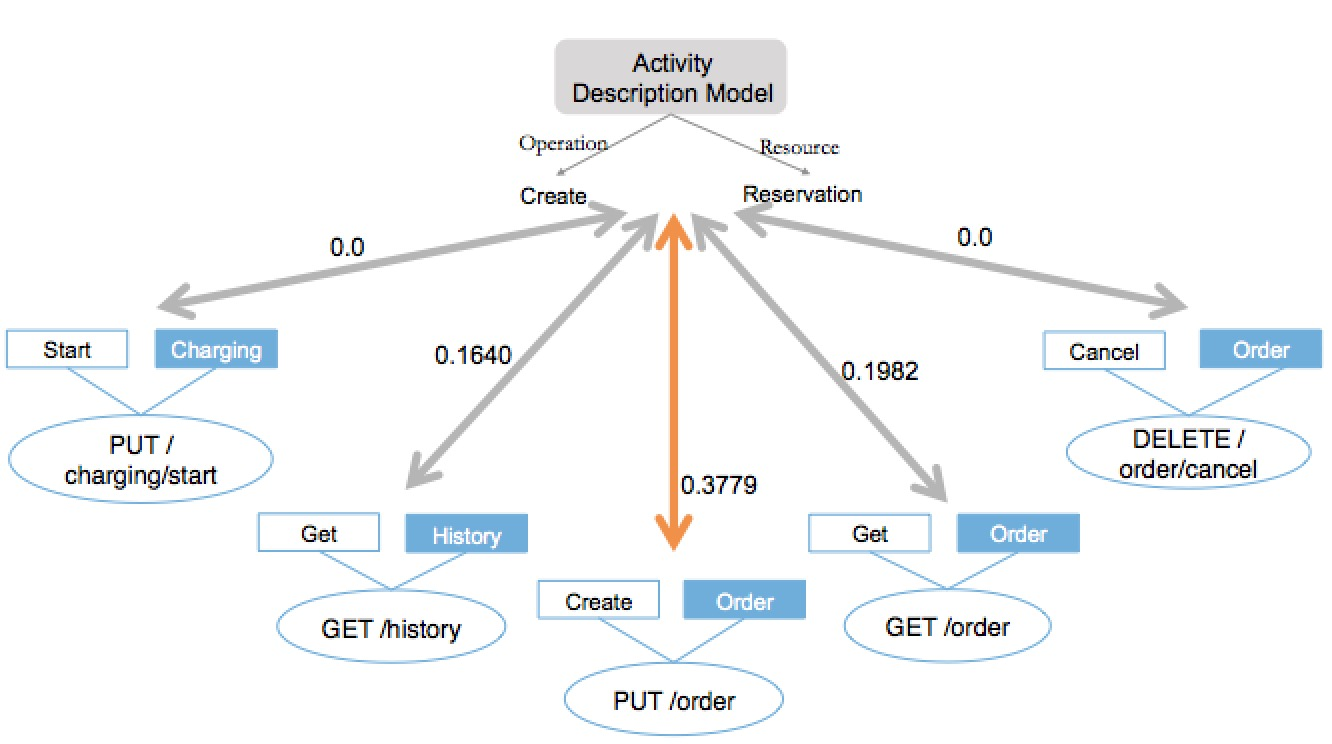
\includegraphics[width=1.0\linewidth]{./graph/matching}
% where an .eps filename suffix will be assumed under latex, 
% and a .pdf suffix will be assumed for pdflatex; or what has been declared
%via \DeclareGraphicsExtensions.
\caption{Matching result of a charging pile example.}
\label{fig_matching}
\end{figure}

A prototype application of the algorithm is implemented. Since there is no open colloction of WoT services to verify the precision of our matching, we have made a simple example for testing. Some RESTful services of the intelligent charging pile is obtained from an existing platform, and a matching result is shown in Fig.~\ref{fig_matching}. By using the WordNet, we calculate the similarity between five services and our functionality defined in Fig.~\ref{fig_activitydescriptionmodeldemo}. The "PUT /order" service is choosed to be the matching service because of the highest similarity, which is actually the operation to add a new reservation. However, there are several domain specified concepts that can not be retrieved in the WordNet, which may cause some wrong computing results. Therefore, a domain specified ontology repository is more suggested to optimize the matching accuracy. 

\subsection{General Service Model}
After the matching service is found, the following question arises:"How to generate a device-independent service with services on the device". 

An important factor to solve this question is to find the corresponding relation between the message description of the activity and the parameters of the services. For services with similar capabilities in various equipement environments, the form of passing arguments might be different. As an example, when querying for the same resource, the name and order of the query conditions might be different in different devices. 

Nevertheless, even if the representation is different, the data type and the semantic meaning of those parameters are consistent. Since the structures of the parameter description in our model and WADL are both consist of a name attribute and a data type attribute, the semantic based matching method is still a feasible solution. The semantic similarity calculation formula between two parameter descriptions is: 
\begin{equation}
    Sim(P_1, P_2)=
   \begin{cases}
   0 &\mbox{if $t_1$ and $t_2$ are not analogous}\\
   S(n_1, n_2) &\mbox{if $t_1$ and $t_2$ are analogous}
   \end{cases}
\end{equation}
where $t_1$ and $t_2$ are the data types of parameter description $P_1$ and $P_2$, and $n_1$ and $n_2$ are name of two parameters. A metrix can be predefined to check whether two data types are analogous(e.g., string and varchar are analogous but integer and date are not).

\begin{figure}[!b]
\centering
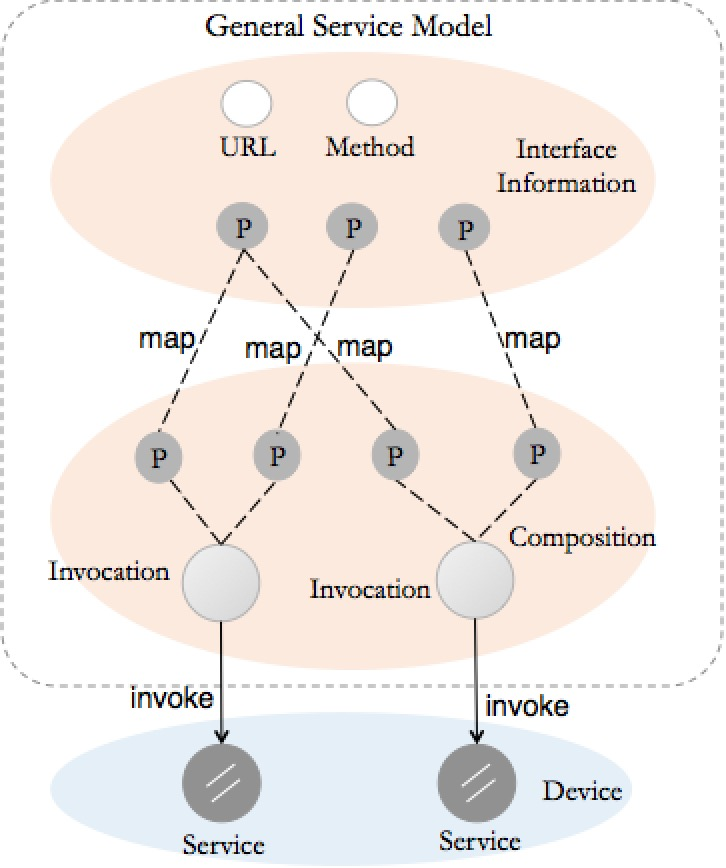
\includegraphics[width=1.0\linewidth]{./graph/generalservicemodel}
% where an .eps filename suffix will be assumed under latex, 
% and a .pdf suffix will be assumed for pdflatex; or what has been declared
%via \DeclareGraphicsExtensions.
\caption{Conception of the general service model.}
\label{fig_generalservice}
\end{figure}

As the matching degree of two parameter description is measured, we can now obtain the parameter matching result between our activity description and practical device services. 

In order to generate the device-independent service, we propose a general service model to express the composition of the services that match the business functionalities in an activity. 

A basic concept of the general service model is shown in fig.~\ref{fig_generalservice}. Structurally, the model is organized in two parts. The first part is the interface information of the general service, which defines the API for the composited service that fulfil the business activity. Considering the device-independency, the interface information is generated from the activity description model, including the URL path, the HTTP request method and the description of request and response parameters. The other one is the composition part. In this part, candidate services are listed with details about how to invoke the service and where to find the parameters. 

%generate the service code
 \begin{algorithm}
        \caption{Generate Service Code}
        \begin{algorithmic}[1] 
            \Require a general service model, including $URL$, $method$, input parameters $IP = \{ ip_1, ip_2,\cdots,ip_n\}$, output parameters $OP = \{ op_1, op_2,\cdots,op_n\}$ and invocations $Inv = \{ inv_1, inv_2,\cdots,inv_n\}$
            \Ensure source code of the service
            \State generate the service interface with $URL$ and $method$
            \For {each parameter $ip_i$ in $IP$}
            		\State set up the mapping between input $ip_i$ and content in $URL$
            \EndFor
            \For {each invocation $inv_i$ in $Inv$}
            		\State generate a new HTTP request with interface in $inv_i$ and parameters in $IP$
            		\State set up the mapping between output $OP$ and content in HTTP response
            \EndFor
            \State
            \Return the source code of the service
        \end{algorithmic}
        \label{al_generating}
 \end{algorithm}
 
Assume we need to execute an activity on two different devices. For each device, a general service model is generated. Comparing two models, we can find that the contents of their interface information part are exactly the same, to make the same HTTP request can be directly reused in both devices. On the contrary, the composition parts on two models are device specific, to composite the actual services on the device. 

Since the general service model furnish an abstract description about the service composition, the specific JavaScript code can be generated to implement and deploy the general service on a Node.js server\cite{wotframework}. A rough process for code generation is introduced in Algorithm~\ref{al_generating}. 

The general service provides a device-independent interface to decouple business code from specific device service. Business activity can bind with the general service instead of the original services on the device. When there is an replacement between two different devices, the process can switch to the new device without any modification about the source code. 





\section{Case Study}
\label{CaseStudy}
In this section, a case study is introduced to verify the feasibility and effectiveness of the approaches above. We construct a prototype system, EVER, an intelligent charging pile sharing platform, to illustrate a typical application of our framework. 

As a kind of WoT equipment, intelligent charging pile is connected to the Internet through WIFI or GPRS, offering RESTful services as operation interfaces. In China, charging pile sharing is an emerging area. The owner can make his private charging pile open to the public, and the public can charge their car by paying a certain fee to the owner. The sharing platform brings a win-win pattern, as the lack of public charging pile can be alleviated and the owner can cover the cost of building the charging pile through the income. 

A brief process of charging through the sharing platform has following steps:
\begin{itemize}
\setlength{\itemsep}{1pt}
\setlength{\parskip}{0pt}
\setlength{\parsep}{0pt}
\item When a driver need to charge his car, he can open the App on his smart phone to fetch all the candidate charging piles nearby. 
\item Then, he can choose a pile and check the detail information of it, including suitable car type, available time, charging fee and etc. 
\item If the pile is suitable, he can make a reservation in his App. 
\item After arriving the charging pile, he can scan the QR code on the charging pile to start charging. 
\item When the charging is over, he can stop the charging in his App and get the bill to pay. 
\end{itemize}

During the charging process, several device services are used to perform business functionalities such as making reservation and generating bill. However, as there are hundreds of different charging pile models in the market, how to adapt the business process to all those models is a great challenge. 

Based on our framework, we designed and implemented a sharing platform, EVER, which has a strong adaptability for the cross-devices process reuse. 

\subsection{Application of the framework}
Reviewing the business process of charging, we found that most activities in the process are related to one or more device services. Therefore, with the help of our Eclipse modeling plugin, we have described those activities in the activity description model. An example of those descriptions is introduced in Fig.~\ref{fig_activitydescriptionmodeldemo}. 

\begin{figure}[!t]
\centering
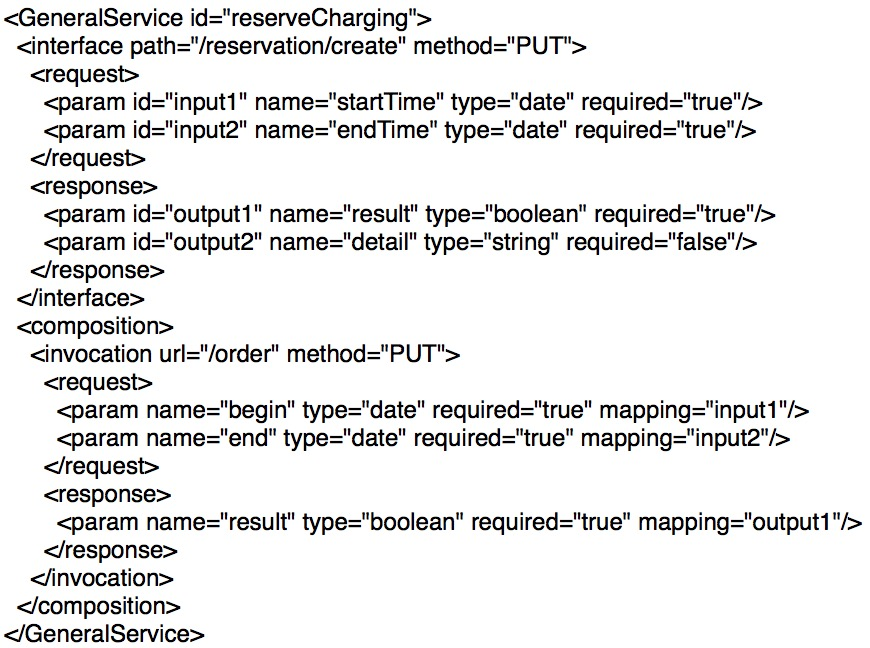
\includegraphics[width=1.0\linewidth]{./graph/generalservicedemo}
% where an .eps filename suffix will be assumed under latex, 
% and a .pdf suffix will be assumed for pdflatex; or what has been declared
%via \DeclareGraphicsExtensions.
\caption{An example of general service model.}
\label{fig_generalservicedemo}
\end{figure}

When a pile owner want to register and share his pile on our platform, the WADL documents of device services should be uploaded. With those descriptions, our matching algorithm is exectued to generate the general service models. Fig.~\ref{fig_generalservicedemo} serves as an example of a general service model.
In the model, the $invocation$ node presents a device service interface for the functionality of reserving charging, which is bound to the general "/reservation/create" service. 

Based on the sample model, source code of the general service can be generated, which is shown in Fig.~\ref{fig_generalservicedemo}. After the general services are deployed on the pile, the pile is now available to the public. 

When a user calls a general service, the general service will help the user to invoke real services on the device. Consequently, our general service offers a device-independent interface to users, which hide all the device services from the user. 

\subsection{Implementation of the system}
EVER is consist of four parts: center server, web site, App and intelligent charging pile. The pile provides RESTful services for the device resources. The center server is in charge of the other APIs of the system. The web site offers user interface for the management of the intelligent charging piles, such as updating the pile state or checking the usage record. Fig.~\ref{fig_prototype1} presents the web page for sharing a new charging pile. The App provides the main charging business. Users can make the reservation, control the charging and pay for bill on the App. The reservation and charging pages of the App is shown in Fig.~\ref{fig_app}. 

\begin{figure}[!t]
\centering
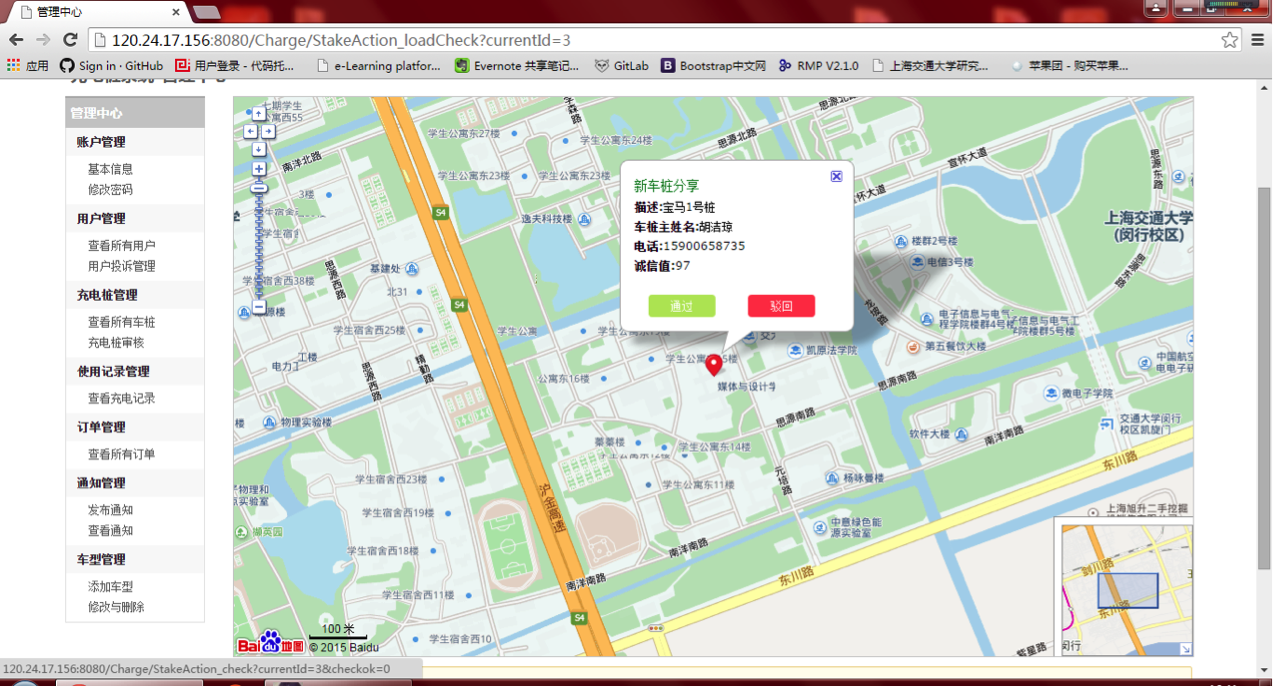
\includegraphics[width=1.0\linewidth]{./graph/prototype1}
% where an .eps filename suffix will be assumed under latex, 
% and a .pdf suffix will be assumed for pdflatex; or what has been declared
%via \DeclareGraphicsExtensions.
\caption{A screenshot of the prototype system.}
\label{fig_prototype1}
\end{figure}

\begin{figure}[!t]
\centering
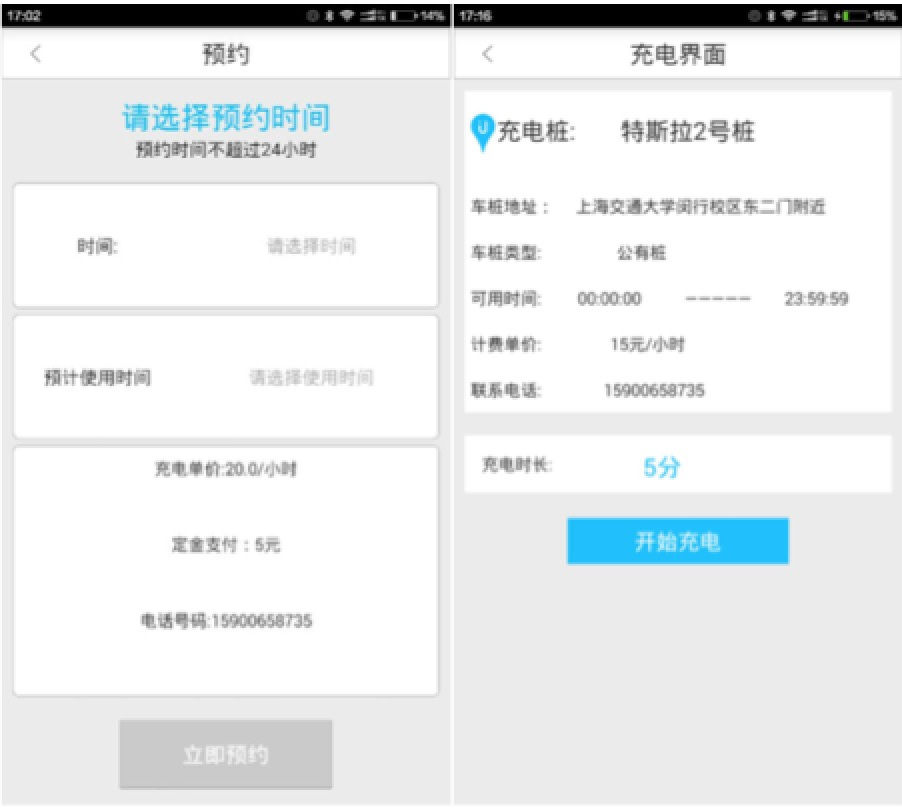
\includegraphics[width=1.0\linewidth]{./graph/app}
% where an .eps filename suffix will be assumed under latex, 
% and a .pdf suffix will be assumed for pdflatex; or what has been declared
%via \DeclareGraphicsExtensions.
\caption{Screenshots of the App.}
\label{fig_app}
\end{figure}



\section{Conclusion}
\label{Conclusion}



% conference papers do not normally have an appendix


% use section* for acknowledgment
\section*{Acknowledgment}


The authors would like to thank...





% trigger a \newpage just before the given reference
% number - used to balance the columns on the last page
% adjust value as needed - may need to be readjusted if
% the document is modified later
%\IEEEtriggeratref{8}
% The "triggered" command can be changed if desired:
%\IEEEtriggercmd{\enlargethispage{-5in}}

% references section

% can use a bibliography generated by BibTeX as a .bbl file
% BibTeX documentation can be easily obtained at:
% http://mirror.ctan.org/biblio/bibtex/contrib/doc/
% The IEEEtran BibTeX style support page is at:
% http://www.michaelshell.org/tex/ieeetran/bibtex/
\bibliographystyle{IEEEtran}
% argument is your BibTeX string definitions and bibliography database(s)
\bibliography{./paper}
%
% <OR> manually copy in the resultant .bbl file
% set second argument of \begin to the number of references
% (used to reserve space for the reference number labels box)





% that's all folks
\end{document}


